\input{Dissertation/appendixsetup}   % Предварительные настройки для правильного подключения Приложений
\chapter{Стабильность межатомных связей в результате моделирования МД белка SOD1} \label{appendix:bstab}

\begin{figure}[ht]
  \center
  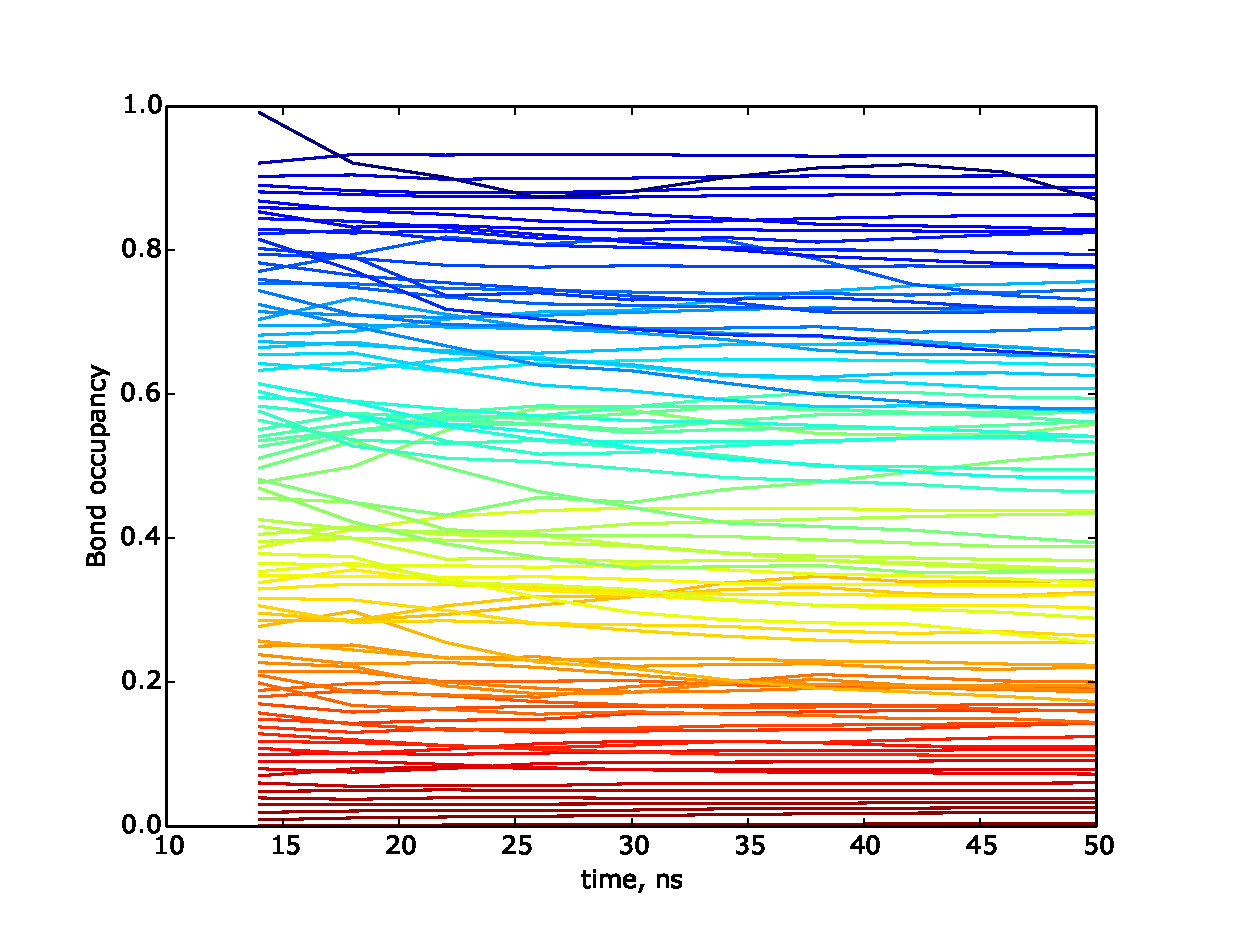
\includegraphics [width=0.75\linewidth] {md_bstab_a}
  \caption{Стабильность водородных связей между атомами белка.}
  \label{img:md_bstab_a}
\end{figure}

\begin{figure}[ht]
  \center
  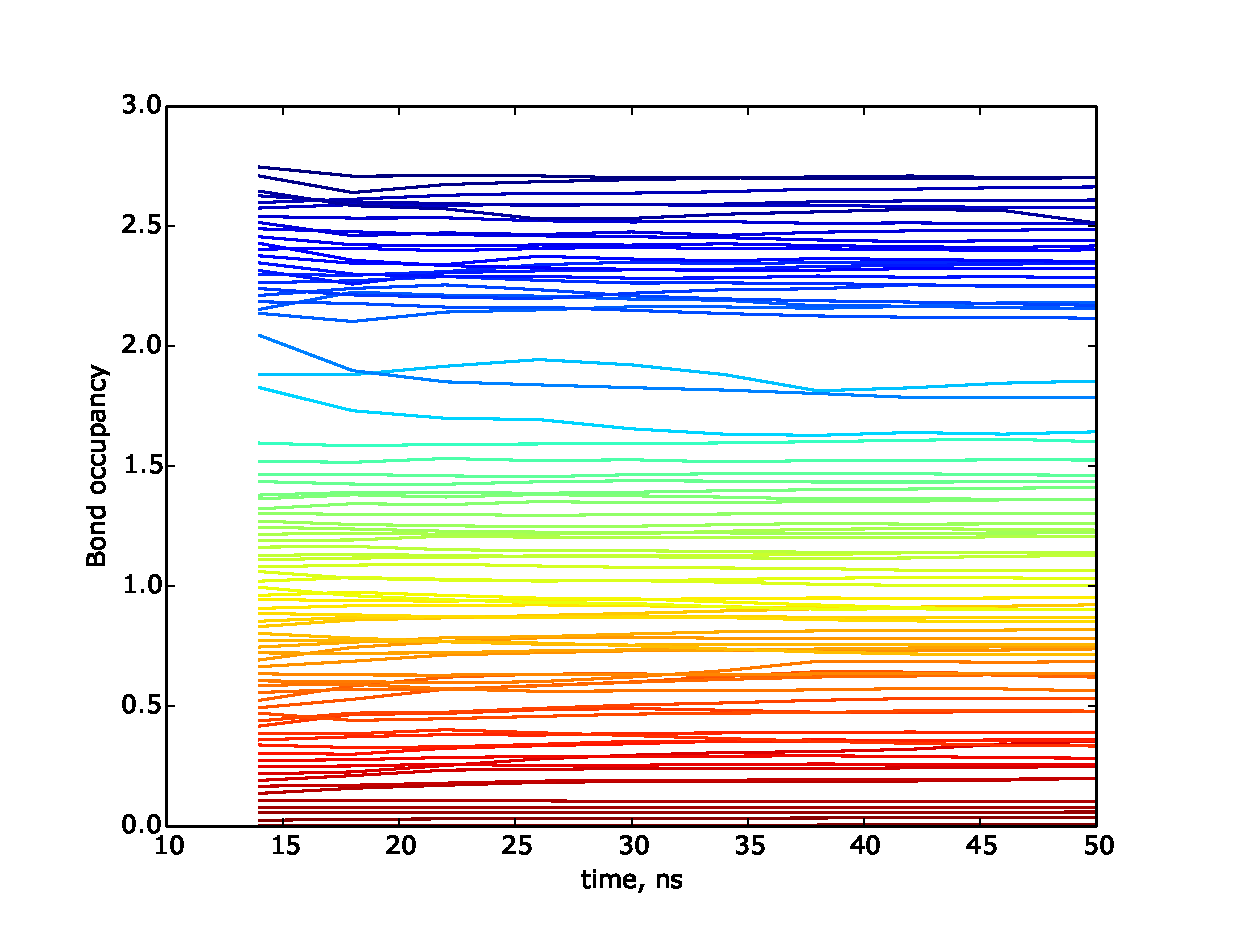
\includegraphics [width=0.75\linewidth] {md_bstab_b}
  \caption{Стабильность водородных связей между атомами белка и атомами молекул воды.}
  \label{img:md_bstab_b}
\end{figure}

\begin{figure}[ht]
  \center
  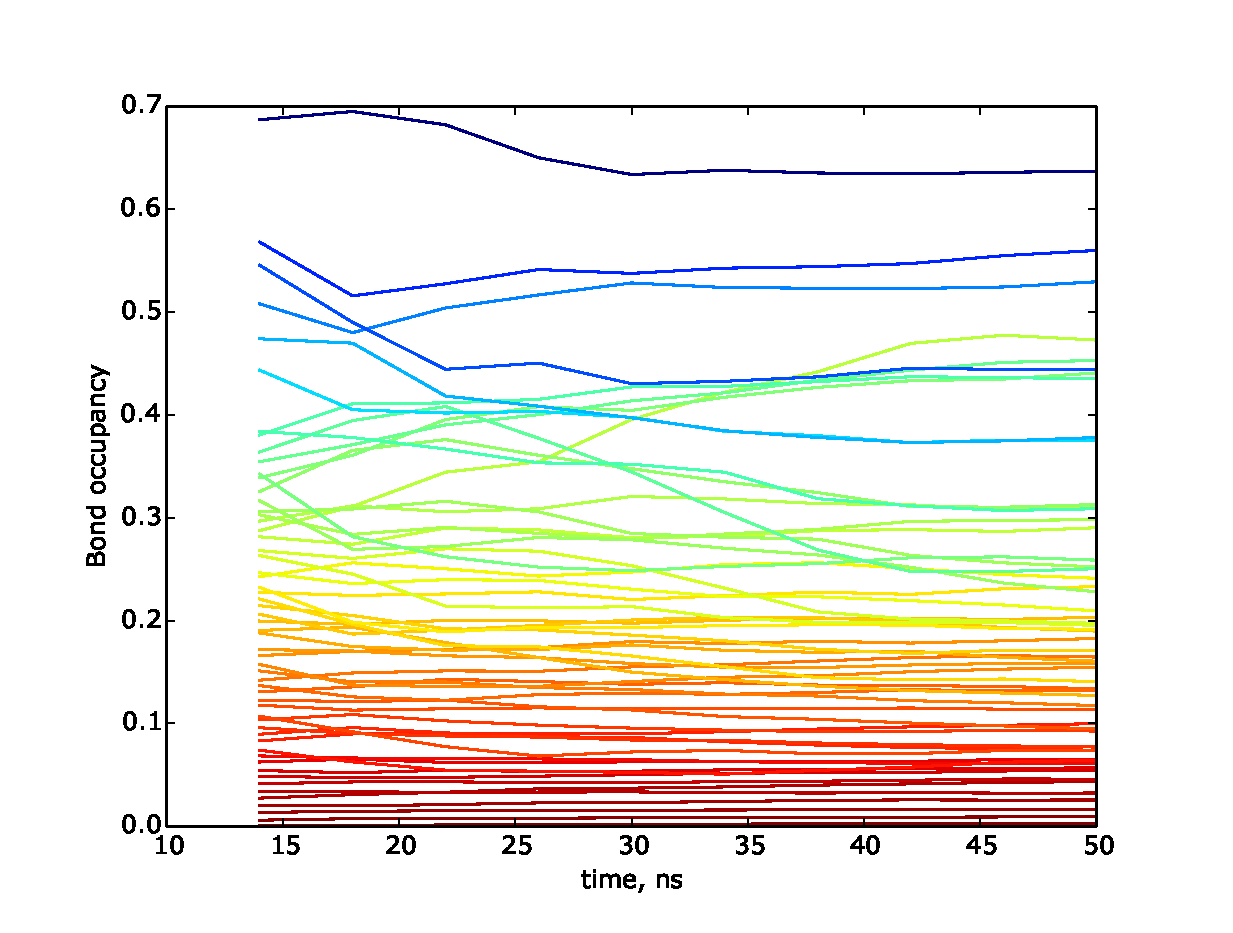
\includegraphics [width=0.75\linewidth] {md_bstab_c}
  \caption{Стабильность водных мостиков.}
  \label{img:md_bstab_c}
\end{figure}

Стабильность связей различного типа между атомами моделируемой системы в зависимости от периода моделирования отображена на Рис. \ref{img:md_bstab_a}, \ref{img:md_bstab_b}, \ref{img:md_bstab_c}. Каждая линия отражает усреднённую динамику времён существования групп связей, имеющих сходную стабильность.
